\documentclass[../main.tex]{subfiles}
\begin{document}
\paragraph{Online solutions}\label{par:poisson_rom}

\begin{figure}[H]
    \centering 
    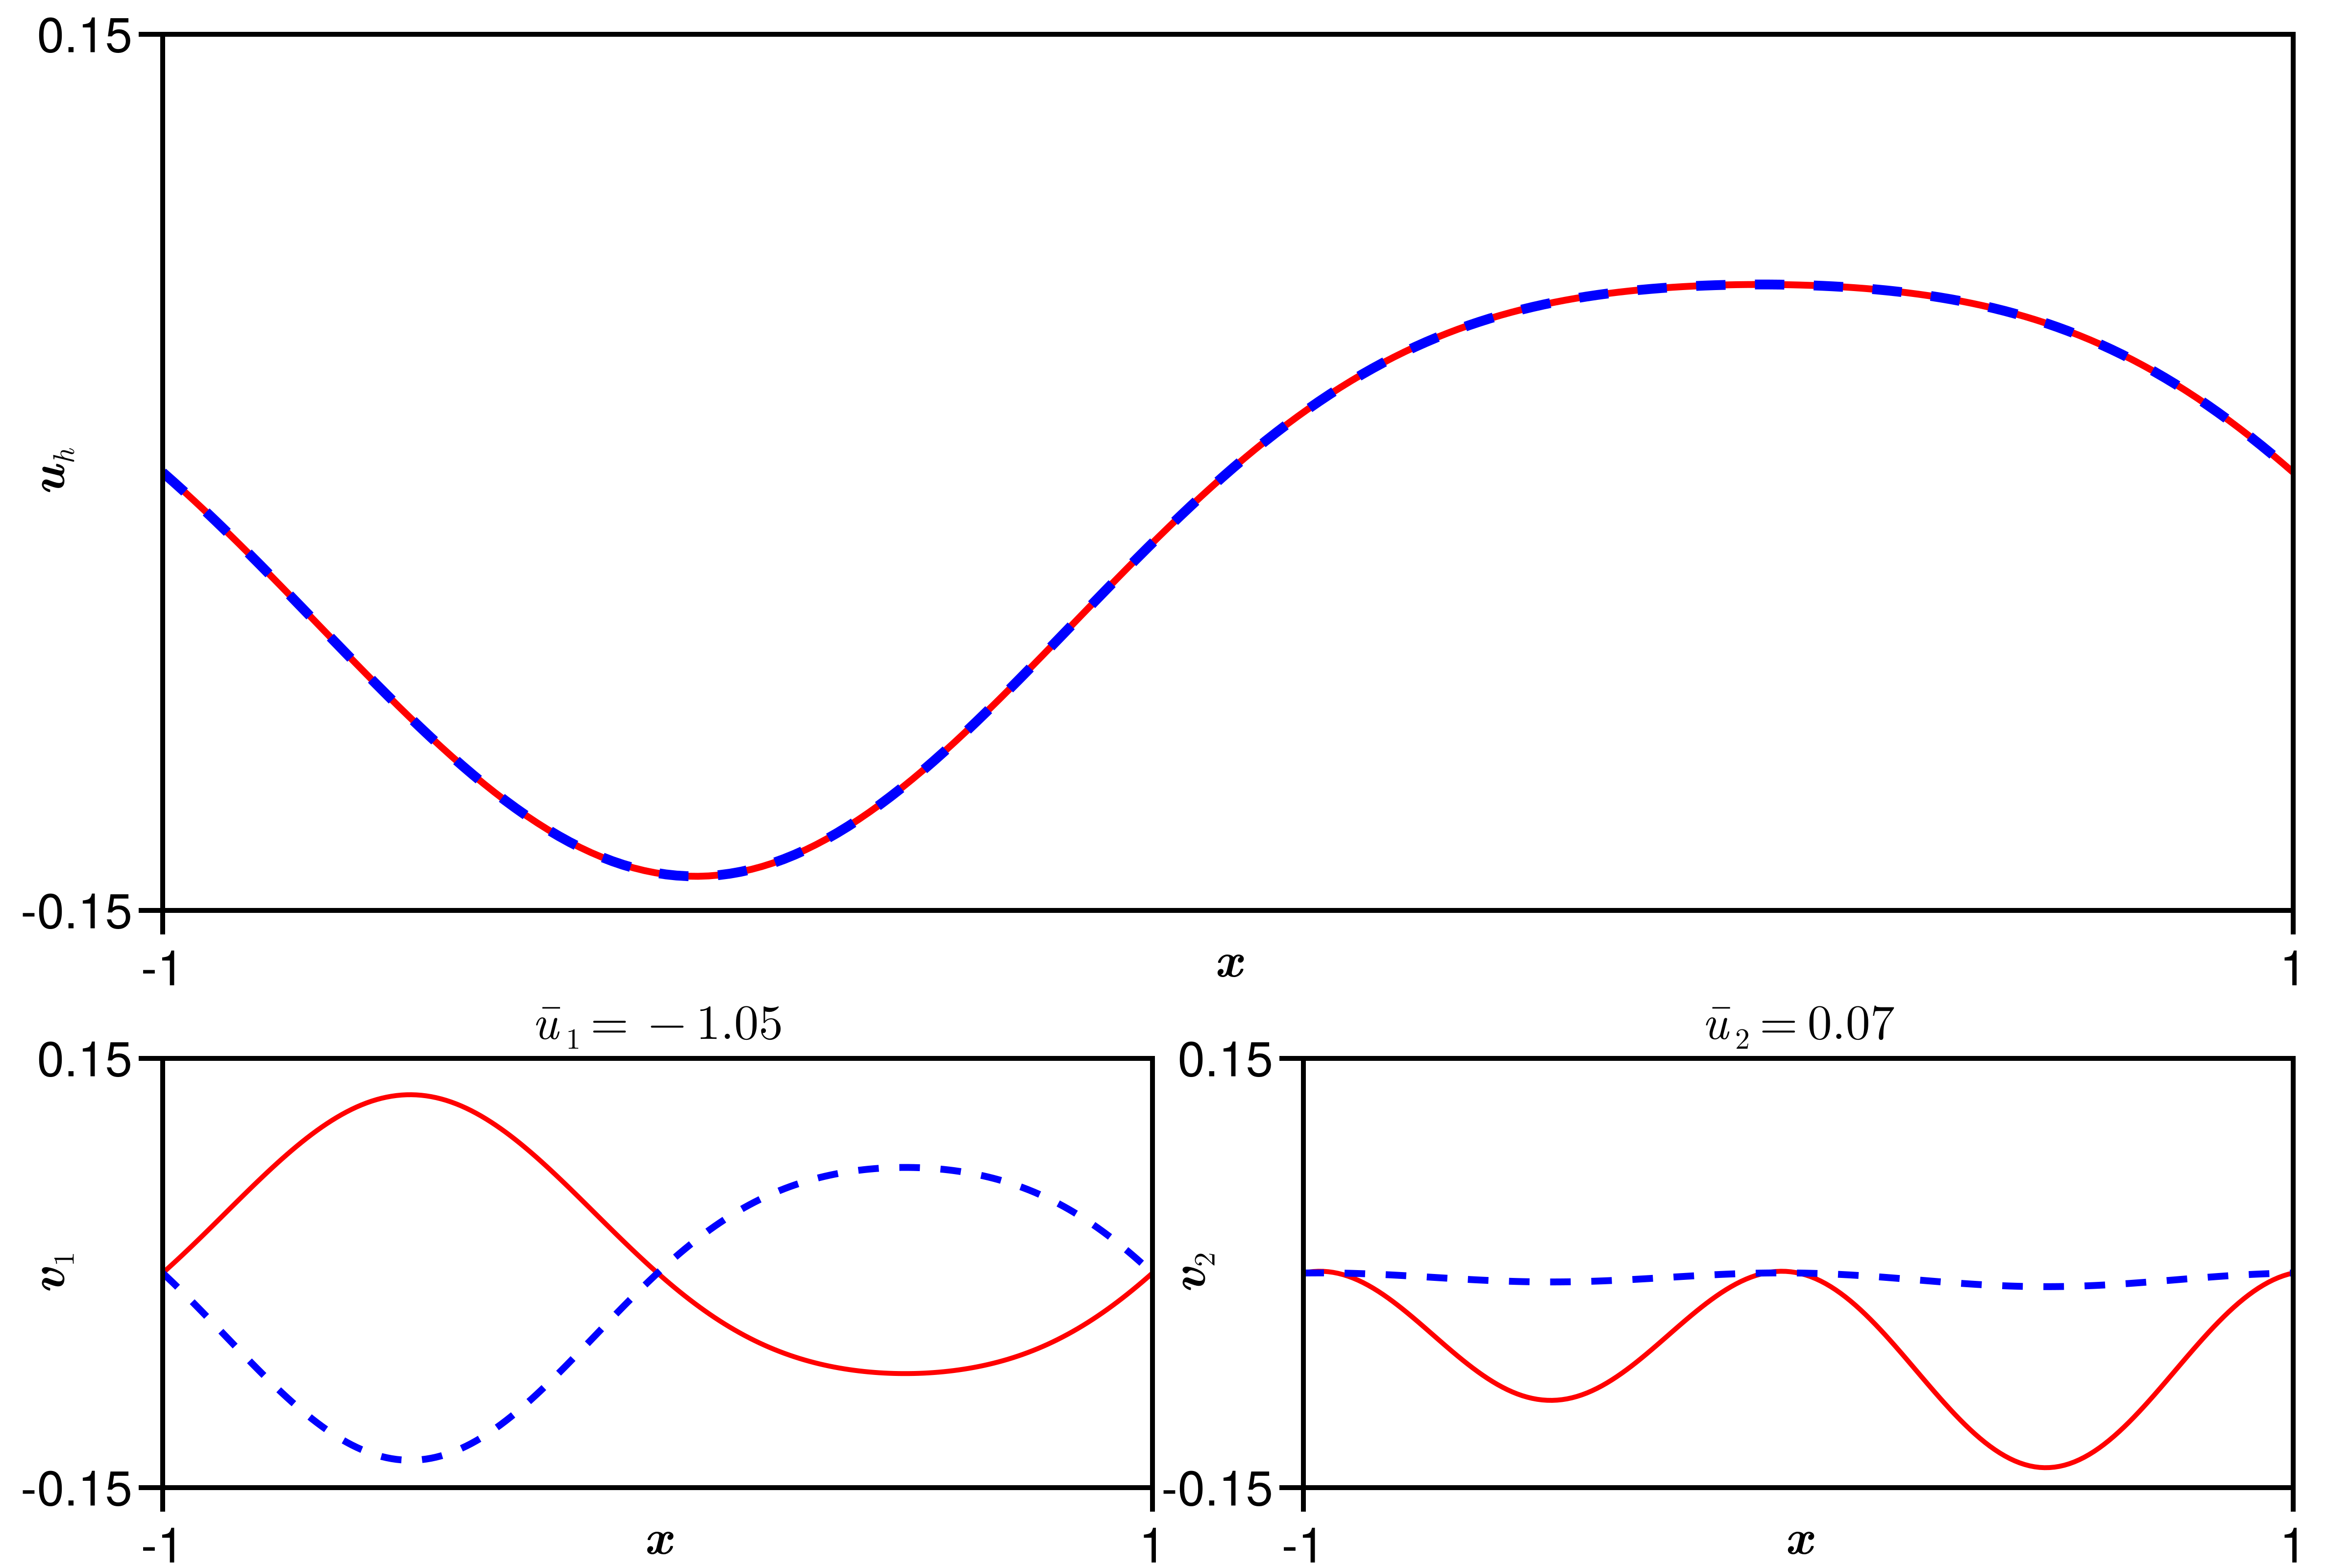
\includegraphics[keepaspectratio, width=0.75\textwidth]{../figures/fig:poisson_rom.png}
    \caption{\textbf{Top}: comparison between the high-order (solid, red) and reduced-order (dashed, blue) solutions at parameter value $\mu=0.73$.
    \textbf{Bottom}: First $2$ singular vectors (solid, red) of the truncated SVD and their weighted representation (dashed, blue) based on the solution $\bar{u}$ of the reduced system (values reported on top of each basis function).}
    \label{fig:poisson_rom}
\end{figure}

Following an homogeneous partition of the domain $\Omega\mapsto\Omega_{h} = \{x\in \Omega\;:\;x = -1 + n \frac{2}{N_{h}}\,,\;n=1,\dots,N_{h}\}$ and by the piecewise linear FE discretisation of the operator, the FOM for \eqref{eq:poisson} reads

\begin{equation*}
     \boldsymbol{A}\boldsymbol{u}_{h} = \boldsymbol{b}\quad\Rightarrow\quad \boldsymbol{u}_{h}=\boldsymbol{A}^{-1}\boldsymbol{b}\,,
\end{equation*}

where $A_{j,k} = \int_{\Omega}^{}\newprime{\varphi_{j}}\newprime{\varphi_{k}}dx$ and $b_{j} = \sin(\pi x_{j}) + \mu\cos(2\pi x_{j})$ with $j=1,\dots,N_{h}$.
Following the offline training phase and the Galerkin projection, the low-dimensional representation of the ROM is

\begin{equation*}
        \boldsymbol{A}\boldsymbol{V}_{r}\bar{\boldsymbol{u}} = \boldsymbol{b}\quad\Rightarrow\quad\bar{\boldsymbol{u}} = \boldsymbol{A}_{r}^{-1}\boldsymbol{b}_{r}\,,
\end{equation*}

where $\boldsymbol{A}_{r} = \boldsymbol{V}_{r}^{T}\boldsymbol{A}\boldsymbol{V}_{r}$ and $\boldsymbol{b}_{r}=\boldsymbol{V}_{r}^{T}\boldsymbol{b}$.
The FOM has $N_{h}=10^{4}$ DOFs and took $\tau_{\,\text{FOM}} = 1.1\cdot10^{-3}$ seconds to compute; the ROM has $N_{r}=2$ DOFs and took $\tau_{\,\text{ROM}} = 0.42\cdot10^{-3}$ seconds to compute.
The \textit{speed-up time} of the ROM is thus $1 - \frac{\tau_{\,\text{ROM}}}{\tau_{\,\text{FOM}}} = 63\%$ i.e. we more than halved the computational time in solving the ROM rather than the FOM at online stage.

\begin{figure}[H]
    \centering 
    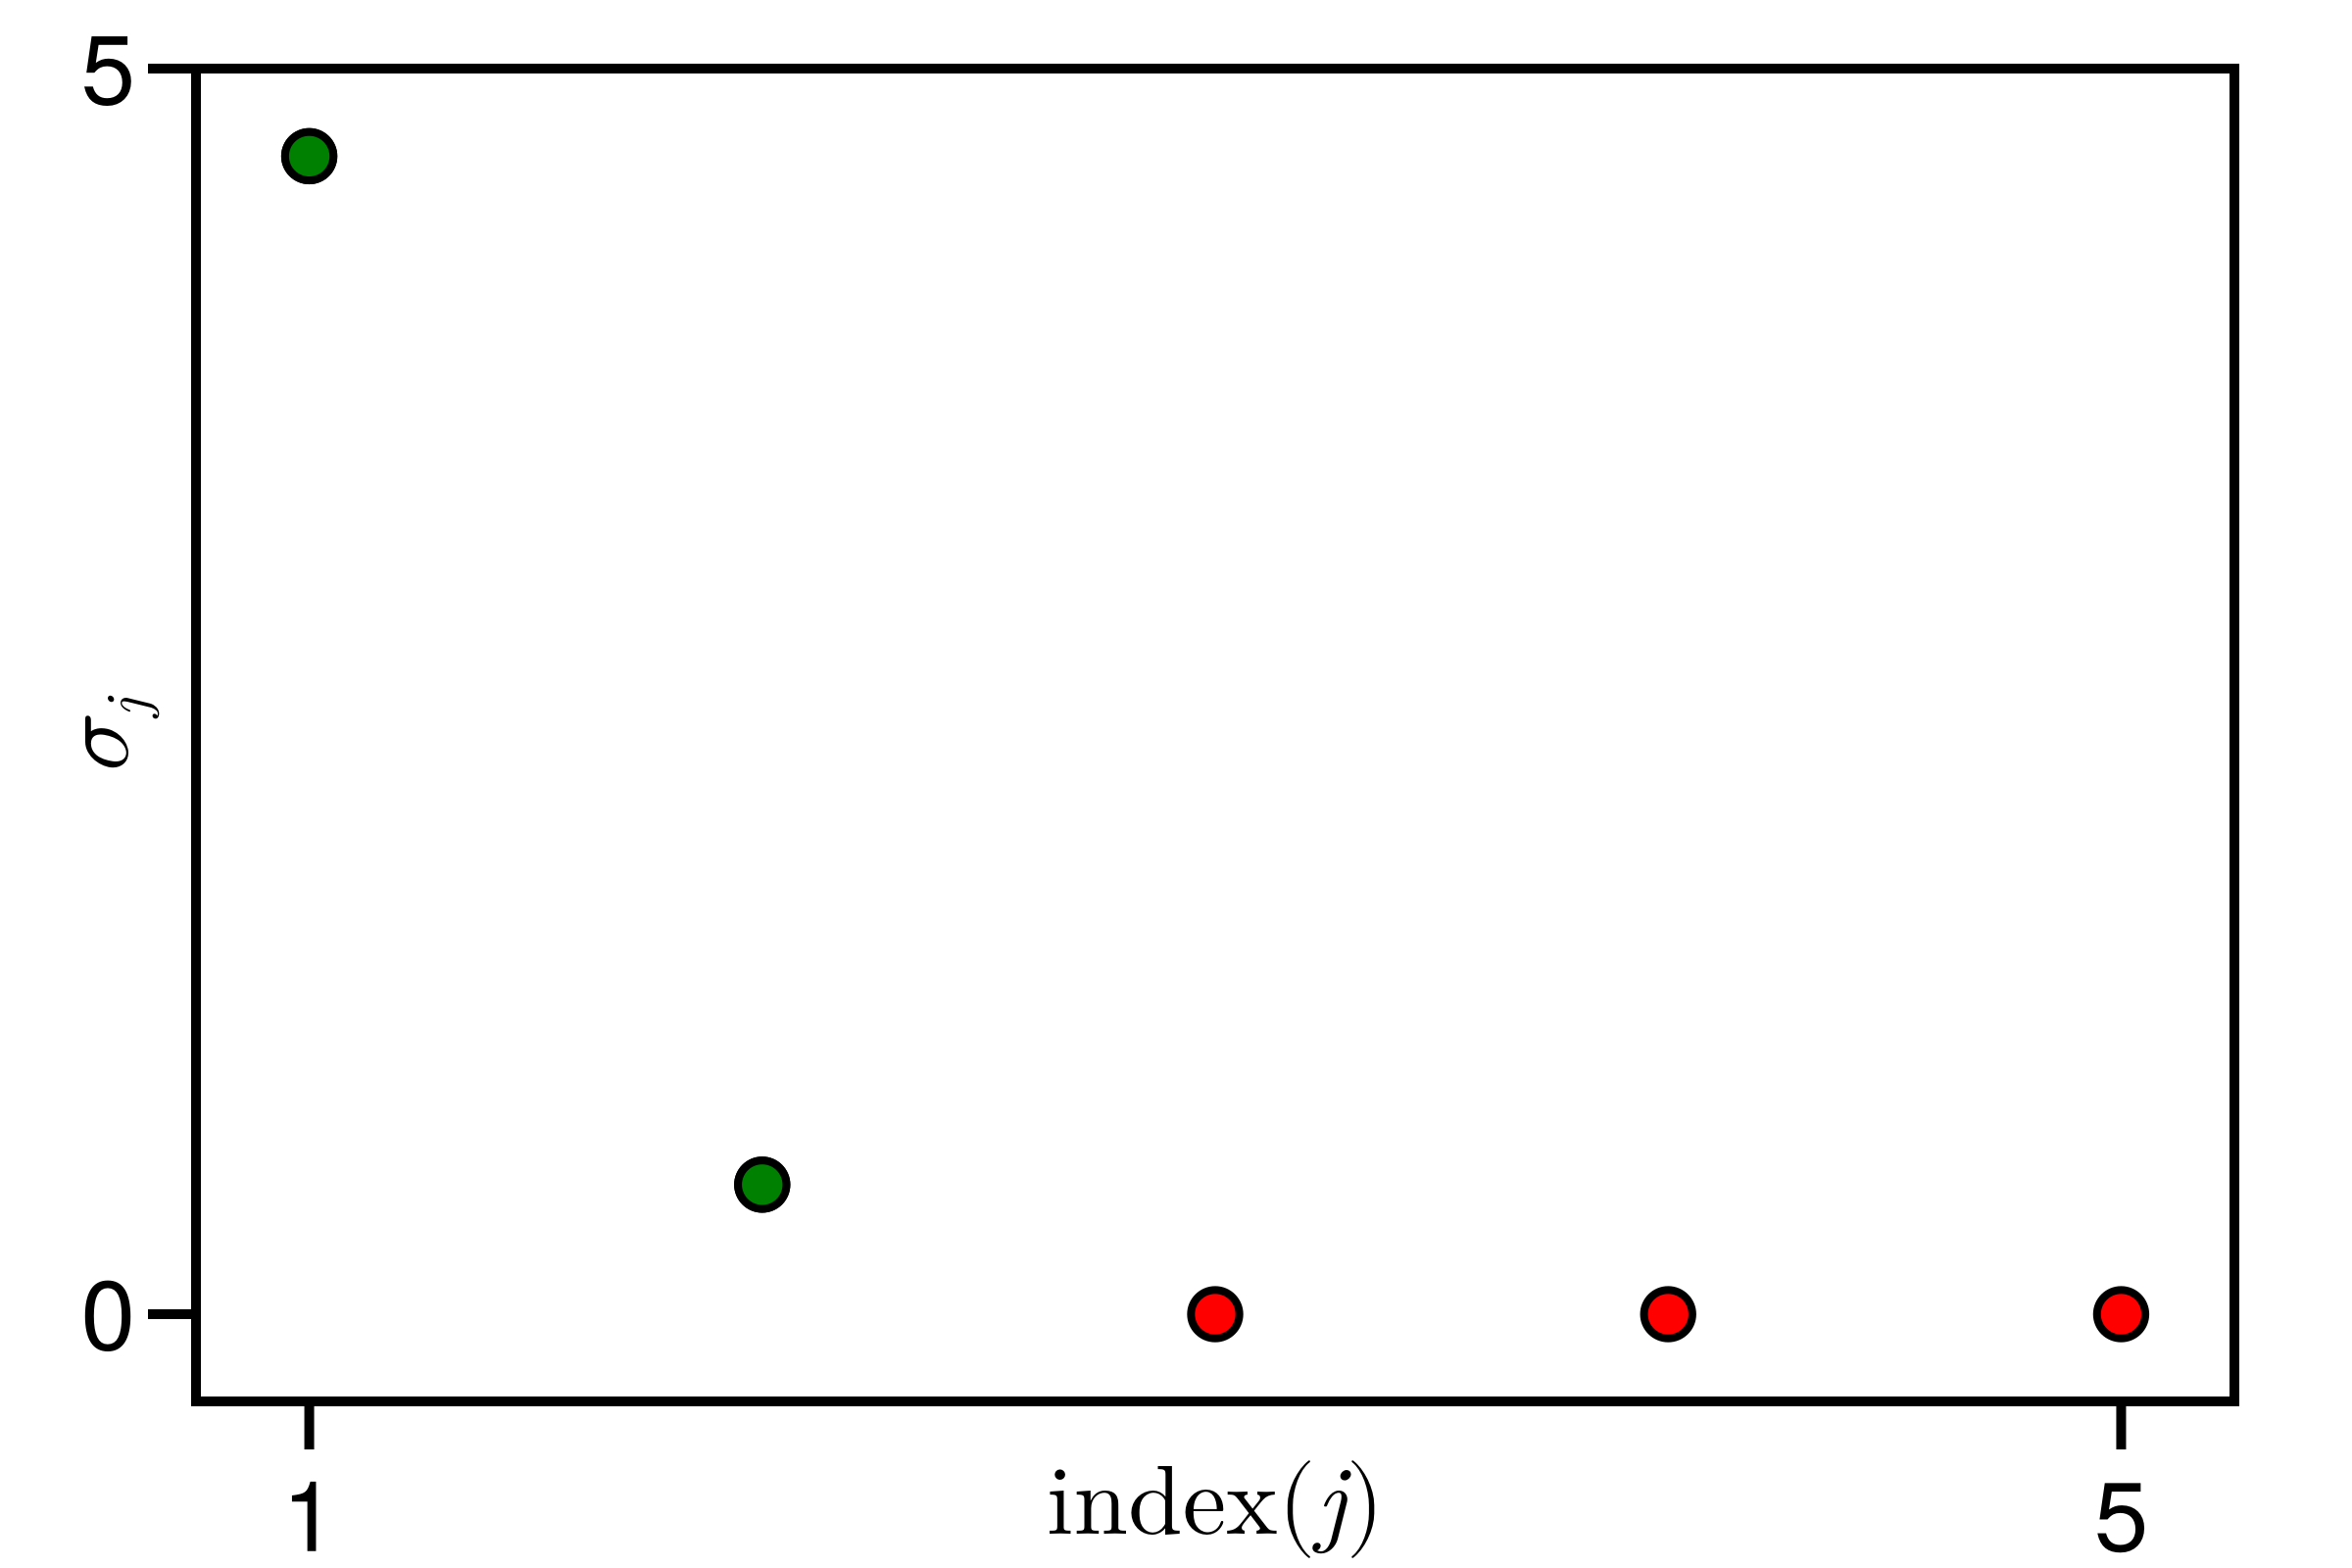
\includegraphics[keepaspectratio, width=0.7\textwidth]{../figures/fig:poisson_decay.png}
    \caption{Kolmogoroff $n-$width decay of \eqref{eq:poisson}. Green dots represent the $N_{r}=2$ singular values used for constructing the ROM solution in Figure \ref{fig:poisson_rom}.}
    \label{fig:poisson_decay}
\end{figure}

\end{document}
